%!TeX root=../tese.tex
%("dica" para o editor de texto: este arquivo é parte de um documento maior)
% para saber mais: https://tex.stackexchange.com/q/78101/183146

%% ------------------------------------------------------------------------- %%
\chapter{Algoritmo guloso}
\label{cap:algoritmo-guloso}

%\definecolor{teste}{rgb}{0.0, 0.3, 0.8}
\definecolor{teste}{rgb}{1,0,0}

Neste capítulo entenderemos como a visão geométrica de um algoritmo de busca em ABB para uma sequência de acessos $X$ se relaciona com o custo ótimo $\OPT(X)$. Além disso, será apresentado um algoritmo guloso offline que transforma um conjunto arboreamente insatisfeito em um conjunto arboreamente satisfeito adicionando uma série de pontos, tentando adicionar o menor número possível de pontos ao conjunto. Por fim, argumentaremos como esse algoritmo pode ser adaptado para um algoritmo online em ABBs dentro do modelo de computação adotado.

\section{Otimalidade} 

Revisemos a definição de custo nesse modelo de computação. O custo para realizar um acesso é o número de nós visitados durante essa operação. Assim, $\OPT(X)$ é o menor custo necessário para um algoritmo de busca offline em ABB realizar todos os acessos de uma entrada $X = (x_{1},\ldots,x_{m})$, ou seja, o número mínimo de visitas a nós necessárias para realizar todos os acessos.

Retornando à análise geométrica, seja $P$ um conjunto de pontos. Denotaremos por \minASS$(P)$ o tamanho do menor conjunto arboreamente satisfeito que contém $P$.

%Seja $P$ a visão geométrica de um algoritmo de busca em ABB que possui custo $\OPT(X)$ para a sequência $X$ de acessos. De acordo com o Lema~\ref{lema:visao_geometrica_vira_ASS}, $P$ é um conjunto arboreamente satisfeito. Além disso, $|P|$ é mínimo para a entrada $X$, pois $P$ é a visão geométrica de um algoritmo de busca em ABB que possui o custo ótimo $\OPT(X)$. Assim, nota-se que $\OPT(X) = \minASS(P_X) = |P|$.

Seja $P$ um menor superconjunto arboreamente satisfeito da visão geométrica da sequência $X$ de acessos, ou seja, $|P| = \minASS(P_X)$. De acordo com o Lema~\ref{lema:ASS_vira_visao_geometrica}, $P$ é a visão geométrica da execução de um algoritmo de busca em ABB. Dentro do contexto de ABBs, $|P|$ representa o número de nós visitados pelo algoritmo de busca e, consequentemente, seu custo dentro do modelo de computação adotado. Por fim, se $|P| = \minASS(P_X)$, então não há nenhum superconjunto arboreamente satisfeito de $P_X$ que possua tamanho menor que $|P|$, ou seja, não há nenhuma execução de um algoritmo de busca que visite menos nós que $|P|$. Assim, concluimos que $|P| = \minASS(P_X) = \OPT(X)$.

%Além disso, de acordo com o modelo de computação, se $P$ possui tamanho $\OPT(X)$, então o algoritmo de 

Isso implica que o problema de encontrar o custo de um algoritmo ótimo de busca em ABB para uma sequência $X$ de acessos pode ser reformulado como o problema de encontrar o menor superconjunto arboreamente satisfeito do conjunto $P_X$.

\section{Guloso futurista}

Apesar de não se saber se é possível encontrar o valor de $\OPT(X)$ em tempo polinomial, e consequentemente encontrar o menor superconjunto de $P_X$ arboreamente satisfeito, apresentaremos o algoritmo Guloso futurista --- Greedy Future --- que dado o conjunto $P_X$ de pontos que representa a sequência $X$ de acessos, produz um conjunto $P$ de pontos pequeno que contém $P_X$ e é arboreamente satisfeito. Esse algoritmo foi descoberto de maneira independente por Lucas \cite{lucas} e por Munro \cite{munro}.

Naturalmente $|P_X| \geq |X| = m$ e todos os pontos de $P_X$ possuem $y$-coordenadas distintas dentro do intervalo $[1,m]$. 

O algoritmo funciona da seguinte maneira: inicialmente defina uma reta horizontal $r$ em $y = 1$ e inicialize $P = P_X$. Seja $a \in P \cap r$ um ponto com coordenadas $(a.x, a.y)$. Para cada $\{a,b\}$-retângulo insatisfeito em $P$, com $b$ um ponto com coordenadas $(b.x, b.y)$, com $b.y < a.y$, adicione a $P$ um ponto em $(b.x, a.y)$. Após satisfazer todos os $\{a,b\}$-retângulos desse tipo, mova $r$ uma unidade para cima e repita. O algoritmo termina após satisfazer todos os $\{a,b\}$-retângulos de $P$ com $r$ em $y = m$. Veja a Figura~\ref{fig:GreedyFuture-funcionamento}.

\begin{figure}
    \centering
    
    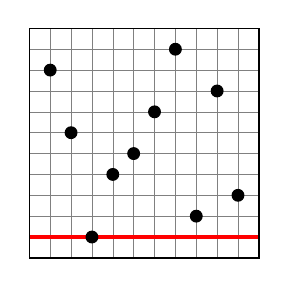
\begin{tikzpicture}[scale=0.265]
        \draw[very thin, gray] (0,0) grid (11,11);
        
        \draw[teste, very thick] (0,1) -- (11,1);

        \filldraw[black] (3,1) circle (8pt);
        \filldraw[black] (8,2) circle (8pt);
        \filldraw[black] (10,3) circle (8pt);
        \filldraw[black] (4,4) circle (8pt);
        \filldraw[black] (5,5) circle (8pt);
        \filldraw[black] (2,6) circle (8pt);
        \filldraw[black] (6,7) circle (8pt);
        \filldraw[black] (9,8) circle (8pt);
        \filldraw[black] (1,9) circle (8pt);
        \filldraw[black] (7,10) circle (8pt);
        \draw[black, line width=0.5pt] (0,0) rectangle (11,11);
    \end{tikzpicture}
    \hfill 
    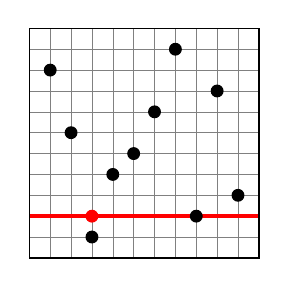
\begin{tikzpicture}[scale=0.265]
        \draw[very thin, gray] (0,0) grid (11,11);
        
        \draw[teste, very thick] (0,2) -- (11,2);

        \filldraw[black] (3,1) circle (8pt);
        \filldraw[black] (8,2) circle (8pt);
        \filldraw[black] (10,3) circle (8pt);
        \filldraw[black] (4,4) circle (8pt);
        \filldraw[black] (5,5) circle (8pt);
        \filldraw[black] (2,6) circle (8pt);
        \filldraw[black] (6,7) circle (8pt);
        \filldraw[black] (9,8) circle (8pt);
        \filldraw[black] (1,9) circle (8pt);
        \filldraw[black] (7,10) circle (8pt);
        \filldraw[teste] (3,2) circle (8pt);

        \draw[black, line width=0.5pt] (0,0) rectangle (11,11);
    \end{tikzpicture}
    \hfill 
    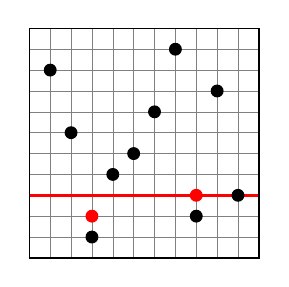
\begin{tikzpicture}[scale=0.265]
        \draw[very thin, gray] (0,0) grid (11,11);
        
        \draw[teste, very thick] (0,3) -- (11,3);

        \filldraw[black] (3,1) circle (8pt);
        \filldraw[black] (8,2) circle (8pt);
        \filldraw[black] (10,3) circle (8pt);
        \filldraw[black] (4,4) circle (8pt);
        \filldraw[black] (5,5) circle (8pt);
        \filldraw[black] (2,6) circle (8pt);
        \filldraw[black] (6,7) circle (8pt);
        \filldraw[black] (9,8) circle (8pt);
        \filldraw[black] (1,9) circle (8pt);
        \filldraw[black] (7,10) circle (8pt);
        \filldraw[teste] (3,2) circle (8pt);
        \filldraw[teste] (8,3) circle (8pt);
        \draw[black, line width=0.5pt] (0,0) rectangle (11,11);
    \end{tikzpicture}
    \hfill 
    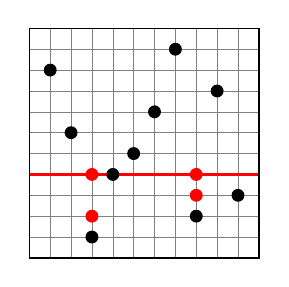
\begin{tikzpicture}[scale=0.265]
        \draw[very thin, gray] (0,0) grid (11,11);
        
        \draw[teste, very thick] (0,4) -- (11,4);

        \filldraw[black] (3,1) circle (8pt);
        \filldraw[black] (8,2) circle (8pt);
        \filldraw[black] (10,3) circle (8pt);
        \filldraw[black] (4,4) circle (8pt);
        \filldraw[black] (5,5) circle (8pt);
        \filldraw[black] (2,6) circle (8pt);
        \filldraw[black] (6,7) circle (8pt);
        \filldraw[black] (9,8) circle (8pt);
        \filldraw[black] (1,9) circle (8pt);
        \filldraw[black] (7,10) circle (8pt);
        \filldraw[teste] (3,2) circle (8pt);
        \filldraw[teste] (8,3) circle (8pt);
        \filldraw[teste] (3,4) circle (8pt);
        \filldraw[teste] (8,4) circle (8pt);
        \draw[black, line width=0.5pt] (0,0) rectangle (11,11); 
    \end{tikzpicture}
    \hfill 
    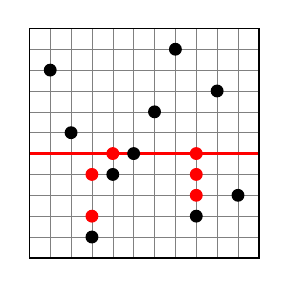
\begin{tikzpicture}[scale=0.265]
        \draw[very thin, gray] (0,0) grid (11,11);
        
        \draw[teste, very thick] (0,5) -- (11,5);

        \filldraw[black] (3,1) circle (8pt);
        \filldraw[black] (8,2) circle (8pt);
        \filldraw[black] (10,3) circle (8pt);
        \filldraw[black] (4,4) circle (8pt);
        \filldraw[black] (5,5) circle (8pt);
        \filldraw[black] (2,6) circle (8pt);
        \filldraw[black] (6,7) circle (8pt);
        \filldraw[black] (9,8) circle (8pt);
        \filldraw[black] (1,9) circle (8pt);
        \filldraw[black] (7,10) circle (8pt);
        \filldraw[teste] (3,2) circle (8pt);
        \filldraw[teste] (8,3) circle (8pt);
        \filldraw[teste] (3,4) circle (8pt);
        \filldraw[teste] (8,4) circle (8pt);
        \filldraw[teste] (4,5) circle (8pt);
        \filldraw[teste] (8,5) circle (8pt);
        \draw[black, line width=0.5pt] (0,0) rectangle (11,11); 
    \end{tikzpicture}
    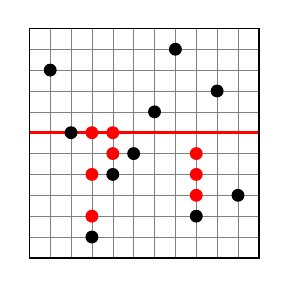
\begin{tikzpicture}[scale=0.265]
        \draw[very thin, gray] (0,0) grid (11,11);
        
        \draw[teste, very thick] (0,6) -- (11,6);

        \filldraw[black] (3,1) circle (8pt);
        \filldraw[black] (8,2) circle (8pt);
        \filldraw[black] (10,3) circle (8pt);
        \filldraw[black] (4,4) circle (8pt);
        \filldraw[black] (5,5) circle (8pt);
        \filldraw[black] (2,6) circle (8pt);
        \filldraw[black] (6,7) circle (8pt);
        \filldraw[black] (9,8) circle (8pt);
        \filldraw[black] (1,9) circle (8pt);
        \filldraw[black] (7,10) circle (8pt);
        \filldraw[teste] (3,2) circle (8pt);
        \filldraw[teste] (8,3) circle (8pt);
        \filldraw[teste] (3,4) circle (8pt);
        \filldraw[teste] (8,4) circle (8pt);
        \filldraw[teste] (4,5) circle (8pt);
        \filldraw[teste] (8,5) circle (8pt);
        \filldraw[teste] (3,6) circle (8pt);
        \filldraw[teste] (4,6) circle (8pt);
        \draw[black, line width=0.5pt] (0,0) rectangle (11,11); 
    \end{tikzpicture}
    \hfill 
    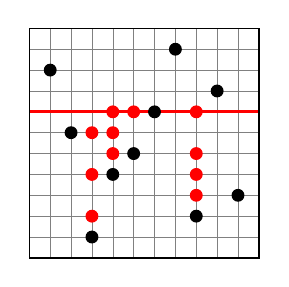
\begin{tikzpicture}[scale=0.265]
        \draw[very thin, gray] (0,0) grid (11,11);
        
        \draw[teste, very thick] (0,7) -- (11,7);

        \filldraw[black] (3,1) circle (8pt);
        \filldraw[black] (8,2) circle (8pt);
        \filldraw[black] (10,3) circle (8pt);
        \filldraw[black] (4,4) circle (8pt);
        \filldraw[black] (5,5) circle (8pt);
        \filldraw[black] (2,6) circle (8pt);
        \filldraw[black] (6,7) circle (8pt);
        \filldraw[black] (9,8) circle (8pt);
        \filldraw[black] (1,9) circle (8pt);
        \filldraw[black] (7,10) circle (8pt);
        \filldraw[teste] (3,2) circle (8pt);
        \filldraw[teste] (8,3) circle (8pt);
        \filldraw[teste] (3,4) circle (8pt);
        \filldraw[teste] (8,4) circle (8pt);
        \filldraw[teste] (4,5) circle (8pt);
        \filldraw[teste] (8,5) circle (8pt);
        \filldraw[teste] (3,6) circle (8pt);
        \filldraw[teste] (4,6) circle (8pt);
        \filldraw[teste] (4,7) circle (8pt);
        \filldraw[teste] (5,7) circle (8pt);
        \filldraw[teste] (8,7) circle (8pt);
        \draw[black, line width=0.5pt] (0,0) rectangle (11,11); 
    \end{tikzpicture}
    \hfill 
    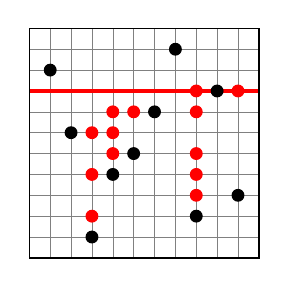
\begin{tikzpicture}[scale=0.265]
        \draw[very thin, gray] (0,0) grid (11,11);
        
        \draw[teste, very thick] (0,8) -- (11,8);

        \filldraw[black] (3,1) circle (8pt);
        \filldraw[black] (8,2) circle (8pt);
        \filldraw[black] (10,3) circle (8pt);
        \filldraw[black] (4,4) circle (8pt);
        \filldraw[black] (5,5) circle (8pt);
        \filldraw[black] (2,6) circle (8pt);
        \filldraw[black] (6,7) circle (8pt);
        \filldraw[black] (9,8) circle (8pt);
        \filldraw[black] (1,9) circle (8pt);
        \filldraw[black] (7,10) circle (8pt);
        \filldraw[teste] (3,2) circle (8pt);
        \filldraw[teste] (8,3) circle (8pt);
        \filldraw[teste] (3,4) circle (8pt);
        \filldraw[teste] (8,4) circle (8pt);
        \filldraw[teste] (4,5) circle (8pt);
        \filldraw[teste] (8,5) circle (8pt);
        \filldraw[teste] (3,6) circle (8pt);
        \filldraw[teste] (4,6) circle (8pt);
        \filldraw[teste] (4,7) circle (8pt);
        \filldraw[teste] (5,7) circle (8pt);
        \filldraw[teste] (8,7) circle (8pt);
        \filldraw[teste] (8,8) circle (8pt);
        \filldraw[teste] (10,8) circle (8pt);
        \draw[black, line width=0.5pt] (0,0) rectangle (11,11); 
    \end{tikzpicture}
    \hfill 
    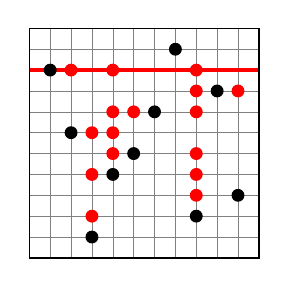
\begin{tikzpicture}[scale=0.265]
        \draw[very thin, gray] (0,0) grid (11,11);
        
        \draw[teste, very thick] (0,9) -- (11,9);

        \filldraw[black] (3,1) circle (8pt);
        \filldraw[black] (8,2) circle (8pt);
        \filldraw[black] (10,3) circle (8pt);
        \filldraw[black] (4,4) circle (8pt);
        \filldraw[black] (5,5) circle (8pt);
        \filldraw[black] (2,6) circle (8pt);
        \filldraw[black] (6,7) circle (8pt);
        \filldraw[black] (9,8) circle (8pt);
        \filldraw[black] (1,9) circle (8pt);
        \filldraw[black] (7,10) circle (8pt);
        \filldraw[teste] (3,2) circle (8pt);
        \filldraw[teste] (8,3) circle (8pt);
        \filldraw[teste] (3,4) circle (8pt);
        \filldraw[teste] (8,4) circle (8pt);
        \filldraw[teste] (4,5) circle (8pt);
        \filldraw[teste] (8,5) circle (8pt);
        \filldraw[teste] (3,6) circle (8pt);
        \filldraw[teste] (4,6) circle (8pt);
        \filldraw[teste] (4,7) circle (8pt);
        \filldraw[teste] (5,7) circle (8pt);
        \filldraw[teste] (8,7) circle (8pt);
        \filldraw[teste] (8,8) circle (8pt);
        \filldraw[teste] (10,8) circle (8pt);
        \filldraw[teste] (2,9) circle (8pt);
        \filldraw[teste] (4,9) circle (8pt);
        \filldraw[teste] (8,9) circle (8pt);
        \draw[black, line width=0.5pt] (0,0) rectangle (11,11); 
    \end{tikzpicture}
    \hfill 
    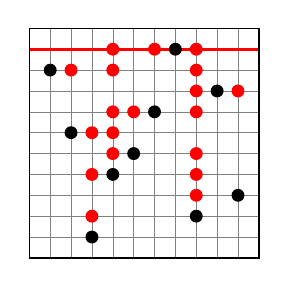
\begin{tikzpicture}[scale=0.265]
        % Desenha o quadriculado
        \draw[very thin, gray] (0,0) grid (11,11);
        
        \draw[teste, very thick] (0,10) -- (11,10);

        \filldraw[black] (3,1) circle (8pt);
        \filldraw[black] (8,2) circle (8pt);
        \filldraw[black] (10,3) circle (8pt);
        \filldraw[black] (4,4) circle (8pt);
        \filldraw[black] (5,5) circle (8pt);
        \filldraw[black] (2,6) circle (8pt);
        \filldraw[black] (6,7) circle (8pt);
        \filldraw[black] (9,8) circle (8pt);
        \filldraw[black] (1,9) circle (8pt);
        \filldraw[black] (7,10) circle (8pt);
        \filldraw[teste] (3,2) circle (8pt);
        \filldraw[teste] (8,3) circle (8pt);
        \filldraw[teste] (3,4) circle (8pt);
        \filldraw[teste] (8,4) circle (8pt);
        \filldraw[teste] (4,5) circle (8pt);
        \filldraw[teste] (8,5) circle (8pt);
        \filldraw[teste] (3,6) circle (8pt);
        \filldraw[teste] (4,6) circle (8pt);
        \filldraw[teste] (4,7) circle (8pt);
        \filldraw[teste] (5,7) circle (8pt);
        \filldraw[teste] (8,7) circle (8pt);
        \filldraw[teste] (8,8) circle (8pt);
        \filldraw[teste] (10,8) circle (8pt);
        \filldraw[teste] (2,9) circle (8pt);
        \filldraw[teste] (4,9) circle (8pt);
        \filldraw[teste] (8,9) circle (8pt);
        \filldraw[teste] (4,10) circle (8pt);
        \filldraw[teste] (8,10) circle (8pt);
        \filldraw[teste] (6,10) circle (8pt);
        \draw[black, line width=0.5pt] (0,0) rectangle (11,11); 
    \end{tikzpicture}
    \caption{Execução do Greedy Future para a sequência X = (3,8,10,4,5,2,6,9,1,7) de acessos.}
\label{fig:GreedyFuture-funcionamento}
\end{figure}

O algoritmo mantém o invariante que, ao final da iteração do algoritmo para a reta horizontal $y = l$, todos os pares de ponto $\{a,b\}$, com $a,b \in P$ e $a.y, b.y \leq l$ são arboreamente satisfeitos. Assim, por construção, o resultado do algoritmo é um conjunto arboreamente satisfeito.

O comportamento desse algoritmo é caracterizado por uma abordagem gulosa local. Esse algoritmo, quando refletido no contexto de ABBs, visita apenas os nós que estão no caminho da raiz até o nó com chave buscada e reorganiza todos os nós visitados de maneira a deixar mais perto da raiz, os nós que serão visitados mais cedo, e consequentemente, mais longe da raiz os nós que serão visitados mais tarde. 

A Figura~\ref{fig:greedy_em_ABB} evidencia este comportamento. A primeira coluna é uma cópia da Figura~\ref{fig:GreedyFuture-funcionamento}. A segunda coluna mostra o caminho utilizado pelo algoritmo de busca para executar o acesso da sequência $X$ e a terceira coluna representa a disposição final da ABB após as rotações serem realizadas preparando-se para os próximos acessos. As ABBs da segunda e terceira coluna estão propositalmente invertidas (com a raiz embaixo e as folhas em cima) para evidenciar que todos os nós visitados em cada acesso (nós em vermelho) são os nós representados pelos pontos na reta $r$ daquele instante.

\begin{figure}
    \centering
    \begin{minipage}[b]{0.48\linewidth}
        \centering
        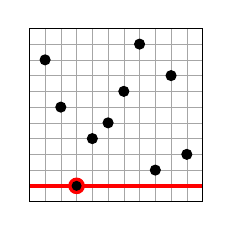
\begin{tikzpicture}[scale=0.2] %1
            \draw[very thin, gray!70] (0,0) grid (11,11);
            
            \draw[teste, line width=1.2pt] (0,1) -- (11,1);
    
            \filldraw[teste] (3,1) circle (14pt);
            \filldraw[black] (3,1) circle (8pt);
            \filldraw[black] (8,2) circle (9pt);
            \filldraw[black] (10,3) circle (9pt);
            \filldraw[black] (4,4) circle (9pt);
            \filldraw[black] (5,5) circle (9pt);
            \filldraw[black] (2,6) circle (9pt);
            \filldraw[black] (6,7) circle (9pt);
            \filldraw[black] (9,8) circle (9pt);
            \filldraw[black] (1,9) circle (9pt);
            \filldraw[black] (7,10) circle (9pt);
            \draw[black, line width=0.5pt] (0,0) rectangle (11,11);
        \end{tikzpicture}
        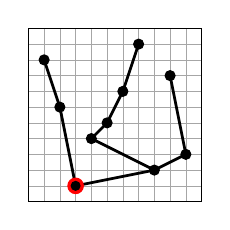
\begin{tikzpicture}[scale=0.2]
            \draw[very thin, gray!70] (0,0) grid (11,11);
            
            \draw[black, line width=1pt] (3,1) -- (8,2) -- (10,3) -- (9,8);
            \draw[black, line width=1pt] (3,1) -- (2,6) -- (1,9);
            \draw[black, line width=1pt] (8,2) -- (4,4) -- (5,5) -- (6,7) -- (7,10);
            
            \filldraw[teste] (3,1) circle (14pt);
            \filldraw[black] (3,1) circle (8pt);
            \filldraw[black] (8,2) circle (9pt);
            \filldraw[black] (10,3) circle (9pt);
            \filldraw[black] (4,4) circle (9pt);
            \filldraw[black] (5,5) circle (9pt);
            \filldraw[black] (2,6) circle (9pt);
            \filldraw[black] (6,7) circle (9pt);
            \filldraw[black] (9,8) circle (9pt);
            \filldraw[black] (1,9) circle (9pt);
            \filldraw[black] (7,10) circle (9pt);
            \draw[black, line width=0.5pt] (0,0) rectangle (11,11);
        \end{tikzpicture}
        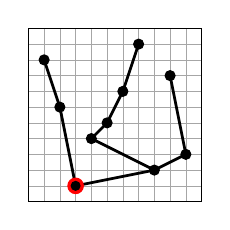
\begin{tikzpicture}[scale=0.2]
            \draw[very thin, gray!70] (0,0) grid (11,11);
            
            \draw[black, line width=1pt] (3,1) -- (8,2) -- (10,3) -- (9,8);
            \draw[black, line width=1pt] (3,1) -- (2,6) -- (1,9);
            \draw[black, line width=1pt] (8,2) -- (4,4) -- (5,5) -- (6,7) -- (7,10);
    
            \filldraw[teste] (3,1) circle (14pt);
            \filldraw[black] (3,1) circle (8pt);
            \filldraw[black] (8,2) circle (9pt);
            \filldraw[black] (10,3) circle (9pt);
            \filldraw[black] (4,4) circle (9pt);
            \filldraw[black] (5,5) circle (9pt);
            \filldraw[black] (2,6) circle (9pt);
            \filldraw[black] (6,7) circle (9pt);
            \filldraw[black] (9,8) circle (9pt);
            \filldraw[black] (1,9) circle (9pt);
            \filldraw[black] (7,10) circle (9pt);
            \draw[black, line width=0.5pt] (0,0) rectangle (11,11);
        \end{tikzpicture}
        \\
        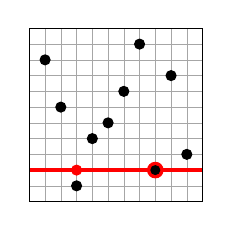
\begin{tikzpicture}[scale=0.2] %2
            \draw[very thin, gray!70] (0,0) grid (11,11);
            
            \draw[teste, line width=1.2pt] (0,2) -- (11,2);
            
    
            \filldraw[black] (3,1) circle (9pt);
            \filldraw[teste] (8,2) circle (14pt);
            \filldraw[black] (8,2) circle (8pt);
            \filldraw[black] (10,3) circle (9pt);
            \filldraw[black] (4,4) circle (9pt);
            \filldraw[black] (5,5) circle (9pt);
            \filldraw[black] (2,6) circle (9pt);
            \filldraw[black] (6,7) circle (9pt);
            \filldraw[black] (9,8) circle (9pt);
            \filldraw[black] (1,9) circle (9pt);
            \filldraw[black] (7,10) circle (9pt);
            \filldraw[teste] (3,2) circle (9pt);
    
            \draw[black, line width=0.5pt] (0,0) rectangle (11,11);
        \end{tikzpicture}
        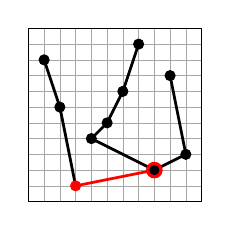
\begin{tikzpicture}[scale=0.2]
            \draw[very thin, gray!70] (0,0) grid (11,11);
            
            \draw[teste, line width=1pt] (3,1) -- (8,2);
            \draw[black, line width=1pt] (8,2) -- (10,3);
            \draw[black, line width=1pt] (10,3) -- (9,8);
            \draw[black, line width=1pt] (3,1) -- (2,6) -- (1,9);
            \draw[black, line width=1pt] (8,2) -- (4,4) -- (5,5) -- (6,7) -- (7,10);
    
            \filldraw[teste] (3,1) circle (9pt);
            \filldraw[teste] (8,2) circle (14pt);
            \filldraw[black] (8,2) circle (8pt);
            \filldraw[black] (10,3) circle (9pt);
            \filldraw[black] (4,4) circle (9pt);
            \filldraw[black] (5,5) circle (9pt);
            \filldraw[black] (2,6) circle (9pt);
            \filldraw[black] (6,7) circle (9pt);
            \filldraw[black] (9,8) circle (9pt);
            \filldraw[black] (1,9) circle (9pt);
            \filldraw[black] (7,10) circle (9pt);
            \draw[black, line width=0.5pt] (0,0) rectangle (11,11);
        \end{tikzpicture}
        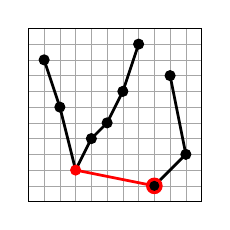
\begin{tikzpicture}[scale=0.2]
            \draw[very thin, gray!70] (0,0) grid (11,11);

            \draw[teste, line width=1pt] (3,2) -- (8,1);
            \draw[black, line width=1pt] (8,1) -- (10,3) -- (9,8);
            \draw[black, line width=1pt] (3,2) -- (2,6) -- (1,9);
            \draw[black, line width=1pt] (3,2) -- (4,4) -- (5,5) -- (6,7) -- (7,10);
            
            \filldraw[teste] (8,1) circle (14pt);
            \filldraw[black] (8,1) circle (8pt);
            \filldraw[teste] (3,2) circle (9pt);
            \filldraw[black] (10,3) circle (9pt);
            \filldraw[black] (4,4) circle (9pt);
            \filldraw[black] (5,5) circle (9pt);
            \filldraw[black] (2,6) circle (9pt);
            \filldraw[black] (6,7) circle (9pt);
            \filldraw[black] (9,8) circle (9pt);
            \filldraw[black] (1,9) circle (9pt);
            \filldraw[black] (7,10) circle (9pt);
            \draw[black, line width=0.5pt] (0,0) rectangle (11,11);
        \end{tikzpicture}
        \\
        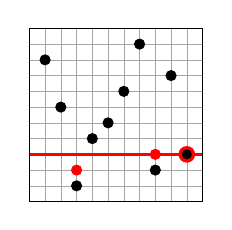
\begin{tikzpicture}[scale=0.2] %3
            \draw[very thin, gray!70] (0,0) grid (11,11);
            
            \draw[teste, line width=1.2pt] (0,3) -- (11,3);
    
            \filldraw[black] (3,1) circle (9pt);
            \filldraw[black] (8,2) circle (9pt);
            \filldraw[teste] (10,3) circle (14pt);
            \filldraw[black] (10,3) circle (8pt);
            \filldraw[black] (4,4) circle (9pt);
            \filldraw[black] (5,5) circle (9pt);
            \filldraw[black] (2,6) circle (9pt);
            \filldraw[black] (6,7) circle (9pt);
            \filldraw[black] (9,8) circle (9pt);
            \filldraw[black] (1,9) circle (9pt);
            \filldraw[black] (7,10) circle (9pt);
            \filldraw[teste] (3,2) circle (9pt);
            \filldraw[teste] (8,3) circle (9pt);
            \draw[black, line width=0.5pt] (0,0) rectangle (11,11);
        \end{tikzpicture}
        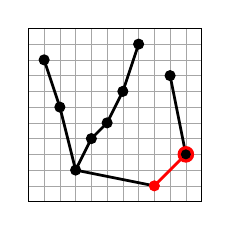
\begin{tikzpicture}[scale=0.2]
            \draw[very thin, gray!70] (0,0) grid (11,11);

            \draw[teste, line width=1pt] (8,1) -- (10,3);
            \draw[black, line width=1pt] (10,3) -- (9,8);
            \draw[black, line width=1pt] (3,2) -- (2,6) -- (1,9);
            \draw[black, line width=1pt] (8,1) -- (3,2) -- (4,4) -- (5,5) -- (6,7) -- (7,10);

            \filldraw[teste] (8,1) circle (9pt);
            \filldraw[black] (3,2) circle (9pt);
            \filldraw[teste] (10,3) circle (14pt);
            \filldraw[black] (10,3) circle (8pt);
            \filldraw[black] (4,4) circle (9pt);
            \filldraw[black] (5,5) circle (9pt);
            \filldraw[black] (2,6) circle (9pt);
            \filldraw[black] (6,7) circle (9pt);
            \filldraw[black] (9,8) circle (9pt);
            \filldraw[black] (1,9) circle (9pt);
            \filldraw[black] (7,10) circle (9pt);
            \draw[black, line width=0.5pt] (0,0) rectangle (11,11);
        \end{tikzpicture}
        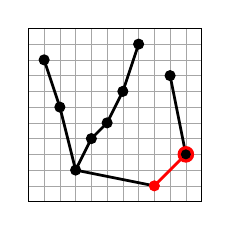
\begin{tikzpicture}[scale=0.2]
            \draw[very thin, gray!70] (0,0) grid (11,11);

            \draw[teste, line width=1pt] (8,1) -- (10,3);
            \draw[black, line width=1pt] (10,3) -- (9,8);
            \draw[black, line width=1pt] (3,2) -- (2,6) -- (1,9);
            \draw[black, line width=1pt] (8,1) -- (3,2) -- (4,4) -- (5,5) -- (6,7) -- (7,10);

            \filldraw[teste] (8,1) circle (9pt);
            \filldraw[black] (3,2) circle (9pt);
            \filldraw[teste] (10,3) circle (14pt);
            \filldraw[black] (10,3) circle (8pt);
            \filldraw[black] (4,4) circle (9pt);
            \filldraw[black] (5,5) circle (9pt);
            \filldraw[black] (2,6) circle (9pt);
            \filldraw[black] (6,7) circle (9pt);
            \filldraw[black] (9,8) circle (9pt);
            \filldraw[black] (1,9) circle (9pt);
            \filldraw[black] (7,10) circle (9pt);
            \draw[black, line width=0.5pt] (0,0) rectangle (11,11);
        \end{tikzpicture}
        \\
        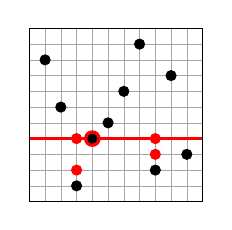
\begin{tikzpicture}[scale=0.2] %4
            \draw[very thin, gray!70] (0,0) grid (11,11);
            
            \draw[teste, line width=1.2pt] (0,4) -- (11,4);
    
            \filldraw[black] (3,1) circle (9pt);
            \filldraw[black] (8,2) circle (9pt);
            \filldraw[black] (10,3) circle (9pt);
            \filldraw[teste] (4,4) circle (14pt);
            \filldraw[black] (4,4) circle (8pt);
            \filldraw[black] (5,5) circle (9pt);
            \filldraw[black] (2,6) circle (9pt);
            \filldraw[black] (6,7) circle (9pt);
            \filldraw[black] (9,8) circle (9pt);
            \filldraw[black] (1,9) circle (9pt);
            \filldraw[black] (7,10) circle (9pt);
            \filldraw[teste] (3,2) circle (9pt);
            \filldraw[teste] (8,3) circle (9pt);
            \filldraw[teste] (3,4) circle (9pt);
            \filldraw[teste] (8,4) circle (9pt);
            \draw[black, line width=0.5pt] (0,0) rectangle (11,11); 
        \end{tikzpicture}
        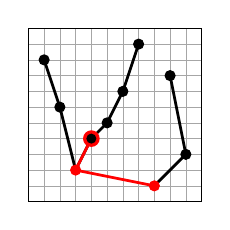
\begin{tikzpicture}[scale=0.2]
            \draw[very thin, gray!70] (0,0) grid (11,11);

            \draw[black, line width=1pt] (8,1) -- (10,3) -- (9,8);
            \draw[black, line width=1pt] (3,2) -- (2,6) -- (1,9);
            \draw[black, line width=1pt] (3,2) -- (4,4) -- (5,5) -- (6,7) -- (7,10);
            \draw[teste, line width=1pt] (8,1) -- (3,2) -- (4,4);

            \filldraw[teste] (8,1) circle (9pt);
            \filldraw[teste] (3,2) circle (9pt);
            \filldraw[black] (10,3) circle (9pt);
            \filldraw[teste] (4,4) circle (14pt);
            \filldraw[black] (4,4) circle (8pt);
            \filldraw[black] (5,5) circle (9pt);
            \filldraw[black] (2,6) circle (9pt);
            \filldraw[black] (6,7) circle (9pt);
            \filldraw[black] (9,8) circle (9pt);
            \filldraw[black] (1,9) circle (9pt);
            \filldraw[black] (7,10) circle (9pt);
            \draw[black, line width=0.5pt] (0,0) rectangle (11,11);
        \end{tikzpicture}
        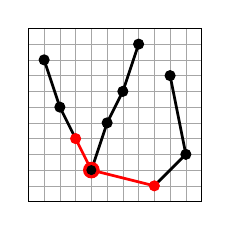
\begin{tikzpicture}[scale=0.2]
            \draw[very thin, gray!70] (0,0) grid (11,11);

            \draw[black, line width=1pt] (8,1) -- (10,3) -- (9,8);
            \draw[black, line width=1pt] (3,4) -- (2,6) -- (1,9);
            \draw[black, line width=1pt] (4,2) -- (5,5) -- (6,7) -- (7,10);
            \draw[teste, line width=1pt] (8,1) -- (4,2) -- (3,4);

            \filldraw[teste] (8,1) circle (9pt);
            \filldraw[teste] (4,2) circle (14pt);
            \filldraw[black] (4,2) circle (8pt);
            \filldraw[black] (10,3) circle (9pt);
            \filldraw[teste] (3,4) circle (9pt);
            \filldraw[black] (5,5) circle (9pt);
            \filldraw[black] (2,6) circle (9pt);
            \filldraw[black] (6,7) circle (9pt);
            \filldraw[black] (9,8) circle (9pt);
            \filldraw[black] (1,9) circle (9pt);
            \filldraw[black] (7,10) circle (9pt);
            \draw[black, line width=0.5pt] (0,0) rectangle (11,11);
        \end{tikzpicture}
        \\
        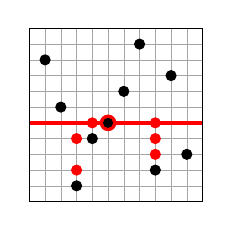
\begin{tikzpicture}[scale=0.2] %5
            \draw[very thin, gray!70] (0,0) grid (11,11);
            
            \draw[teste, line width=1.2pt] (0,5) -- (11,5);
    
            \filldraw[black] (3,1) circle (9pt);
            \filldraw[black] (8,2) circle (9pt);
            \filldraw[black] (10,3) circle (9pt);
            \filldraw[black] (4,4) circle (9pt);
            \filldraw[teste] (5,5) circle (14pt);
            \filldraw[black] (5,5) circle (8pt);
            \filldraw[black] (2,6) circle (9pt);
            \filldraw[black] (6,7) circle (9pt);
            \filldraw[black] (9,8) circle (9pt);
            \filldraw[black] (1,9) circle (9pt);
            \filldraw[black] (7,10) circle (9pt);
            \filldraw[teste] (3,2) circle (9pt);
            \filldraw[teste] (8,3) circle (9pt);
            \filldraw[teste] (3,4) circle (9pt);
            \filldraw[teste] (8,4) circle (9pt);
            \filldraw[teste] (4,5) circle (9pt);
            \filldraw[teste] (8,5) circle (9pt);
            \draw[black, line width=0.5pt] (0,0) rectangle (11,11); 
        \end{tikzpicture}
        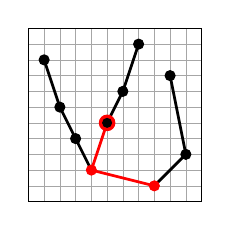
\begin{tikzpicture}[scale=0.2]
            \draw[very thin, gray!70] (0,0) grid (11,11);

            \draw[black, line width=1pt] (8,1) -- (10,3) -- (9,8);
            \draw[black, line width=1pt] (4,2) -- (3,4) -- (2,6) -- (1,9);
            \draw[black, line width=1pt] (5,5) -- (6,7) -- (7,10);
            \draw[teste, line width=1pt] (8,1) -- (4,2) -- (5,5);

            \filldraw[teste] (8,1) circle (9pt);
            \filldraw[teste] (4,2) circle (9pt);
            \filldraw[black] (10,3) circle (9pt);
            \filldraw[black] (3,4) circle (9pt);
            \filldraw[teste] (5,5) circle (14pt);
            \filldraw[black] (5,5) circle (8pt);
            \filldraw[black] (2,6) circle (9pt);
            \filldraw[black] (6,7) circle (9pt);
            \filldraw[black] (9,8) circle (9pt);
            \filldraw[black] (1,9) circle (9pt);
            \filldraw[black] (7,10) circle (9pt);
            \draw[black, line width=0.5pt] (0,0) rectangle (11,11);
        \end{tikzpicture}
        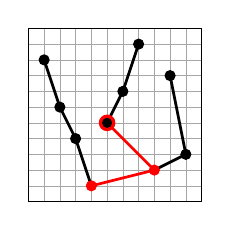
\begin{tikzpicture}[scale=0.2]
            \draw[very thin, gray!70] (0,0) grid (11,11);

            \draw[black, line width=1pt] (8,2) -- (10,3) -- (9,8);
            \draw[black, line width=1pt] (4,1) -- (3,4) -- (2,6) -- (1,9);
            \draw[black, line width=1pt] (5,5) -- (6,7) -- (7,10);
            \draw[teste, line width=1pt] (4,1) -- (8,2) -- (5,5);

            \filldraw[teste] (4,1) circle (9pt);
            \filldraw[teste] (8,2) circle (9pt);
            \filldraw[black] (10,3) circle (9pt);
            \filldraw[black] (3,4) circle (9pt);
            \filldraw[teste] (5,5) circle (14pt);
            \filldraw[black] (5,5) circle (8pt);
            \filldraw[black] (2,6) circle (9pt);
            \filldraw[black] (6,7) circle (9pt);
            \filldraw[black] (9,8) circle (9pt);
            \filldraw[black] (1,9) circle (9pt);
            \filldraw[black] (7,10) circle (9pt);
            \draw[black, line width=0.5pt] (0,0) rectangle (11,11);
        \end{tikzpicture}
    \end{minipage}
    %\hspace{0.01\linewidth}
    \hfill
    \begin{minipage}[b]{0.48\linewidth}
        \centering
        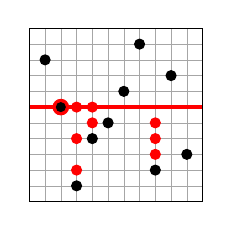
\begin{tikzpicture}[scale=0.2] %6
            \draw[very thin, gray!70] (0,0) grid (11,11);
            
            \draw[teste, line width=1.2pt] (0,6) -- (11,6);
    
            \filldraw[black] (3,1) circle (9pt);
            \filldraw[black] (8,2) circle (9pt);
            \filldraw[black] (10,3) circle (9pt);
            \filldraw[black] (4,4) circle (9pt);
            \filldraw[black] (5,5) circle (9pt);
            \filldraw[teste] (2,6) circle (14pt);
            \filldraw[black] (2,6) circle (8pt);
            \filldraw[black] (6,7) circle (9pt);
            \filldraw[black] (9,8) circle (9pt);
            \filldraw[black] (1,9) circle (9pt);
            \filldraw[black] (7,10) circle (9pt);
            \filldraw[teste] (3,2) circle (9pt);
            \filldraw[teste] (8,3) circle (9pt);
            \filldraw[teste] (3,4) circle (9pt);
            \filldraw[teste] (8,4) circle (9pt);
            \filldraw[teste] (4,5) circle (9pt);
            \filldraw[teste] (8,5) circle (9pt);
            \filldraw[teste] (3,6) circle (9pt);
            \filldraw[teste] (4,6) circle (9pt);
            \draw[black, line width=0.5pt] (0,0) rectangle (11,11); 
        \end{tikzpicture}
        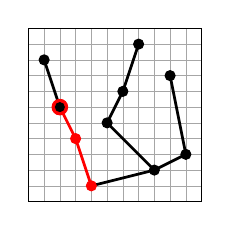
\begin{tikzpicture}[scale=0.2]
            \draw[very thin, gray!70] (0,0) grid (11,11);

            \draw[black, line width=1pt] (8,2) -- (10,3) -- (9,8);
            \draw[teste, line width=1pt] (4,1) -- (3,4) -- (2,6);
            \draw[black, line width=1pt] (2,6) -- (1,9);
            \draw[black, line width=1pt] (5,5) -- (6,7) -- (7,10);
            \draw[black, line width=1pt] (4,1) -- (8,2) -- (5,5);

            \filldraw[teste] (4,1) circle (9pt);
            \filldraw[black] (8,2) circle (9pt);
            \filldraw[black] (10,3) circle (9pt);
            \filldraw[teste] (3,4) circle (9pt);
            \filldraw[black] (5,5) circle (9pt);
            \filldraw[teste] (2,6) circle (14pt);
            \filldraw[black] (2,6) circle (8pt);
            \filldraw[black] (6,7) circle (9pt);
            \filldraw[black] (9,8) circle (9pt);
            \filldraw[black] (1,9) circle (9pt);
            \filldraw[black] (7,10) circle (9pt);
            \draw[black, line width=0.5pt] (0,0) rectangle (11,11);
        \end{tikzpicture}
        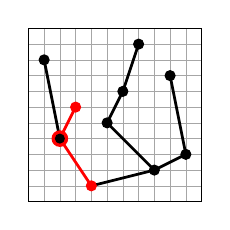
\begin{tikzpicture}[scale=0.2]
            \draw[very thin, gray!70] (0,0) grid (11,11);

            \draw[black, line width=1pt] (8,2) -- (10,3) -- (9,8);
            \draw[teste, line width=1pt] (4,1) -- (2,4) -- (3,6);
            \draw[black, line width=1pt] (2,4) -- (1,9);
            \draw[black, line width=1pt] (5,5) -- (6,7) -- (7,10);
            \draw[black, line width=1pt] (4,1) -- (8,2) -- (5,5);

            \filldraw[teste] (4,1) circle (9pt);
            \filldraw[black] (8,2) circle (9pt);
            \filldraw[black] (10,3) circle (9pt);
            \filldraw[teste] (2,4) circle (14pt);
            \filldraw[black] (2,4) circle (8pt);
            \filldraw[black] (5,5) circle (9pt);
            \filldraw[teste] (3,6) circle (9pt);
            \filldraw[black] (6,7) circle (9pt);
            \filldraw[black] (9,8) circle (9pt);
            \filldraw[black] (1,9) circle (9pt);
            \filldraw[black] (7,10) circle (9pt);
            \draw[black, line width=0.5pt] (0,0) rectangle (11,11);
        \end{tikzpicture}
        \\
        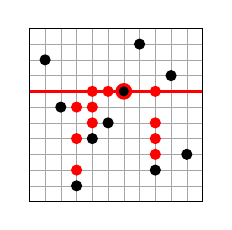
\begin{tikzpicture}[scale=0.2] %7
            \draw[very thin, gray!70] (0,0) grid (11,11);
            
            \draw[teste, line width=1.2pt] (0,7) -- (11,7);
    
            \filldraw[black] (3,1) circle (9pt);
            \filldraw[black] (8,2) circle (9pt);
            \filldraw[black] (10,3) circle (9pt);
            \filldraw[black] (4,4) circle (9pt);
            \filldraw[black] (5,5) circle (9pt);
            \filldraw[black] (2,6) circle (9pt);
            \filldraw[teste] (6,7) circle (14pt);
            \filldraw[black] (6,7) circle (8pt);
            \filldraw[black] (9,8) circle (9pt);
            \filldraw[black] (1,9) circle (9pt);
            \filldraw[black] (7,10) circle (9pt);
            \filldraw[teste] (3,2) circle (9pt);
            \filldraw[teste] (8,3) circle (9pt);
            \filldraw[teste] (3,4) circle (9pt);
            \filldraw[teste] (8,4) circle (9pt);
            \filldraw[teste] (4,5) circle (9pt);
            \filldraw[teste] (8,5) circle (9pt);
            \filldraw[teste] (3,6) circle (9pt);
            \filldraw[teste] (4,6) circle (9pt);
            \filldraw[teste] (4,7) circle (9pt);
            \filldraw[teste] (5,7) circle (9pt);
            \filldraw[teste] (8,7) circle (9pt);
            \draw[black, line width=0.5pt] (0,0) rectangle (11,11); 
        \end{tikzpicture}
        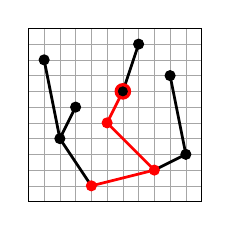
\begin{tikzpicture}[scale=0.2]
            \draw[very thin, gray!70] (0,0) grid (11,11);

            \draw[black, line width=1pt] (8,2) -- (10,3) -- (9,8);
            \draw[black, line width=1pt] (4,1) -- (2,4) -- (3,6);
            \draw[black, line width=1pt] (2,4) -- (1,9);
            \draw[black, line width=1pt] (6,7) -- (7,10);
            \draw[teste, line width=1pt] (4,1) -- (8,2) -- (5,5) -- (6,7);

            \filldraw[teste] (4,1) circle (9pt);
            \filldraw[teste] (8,2) circle (9pt);
            \filldraw[black] (10,3) circle (9pt);
            \filldraw[black] (2,4) circle (9pt);
            \filldraw[teste] (5,5) circle (9pt);
            \filldraw[black] (3,6) circle (9pt);
            \filldraw[teste] (6,7) circle (14pt);
            \filldraw[black] (6,7) circle (8pt);
            \filldraw[black] (9,8) circle (9pt);
            \filldraw[black] (1,9) circle (9pt);
            \filldraw[black] (7,10) circle (9pt);
            \draw[black, line width=0.5pt] (0,0) rectangle (11,11);
        \end{tikzpicture}
        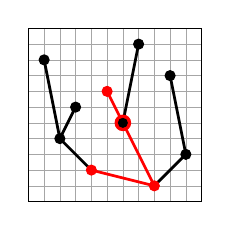
\begin{tikzpicture}[scale=0.2]
            \draw[very thin, gray!70] (0,0) grid (11,11);

            \draw[black, line width=1pt] (8,1) -- (10,3) -- (9,8);
            \draw[black, line width=1pt] (4,2) -- (2,4) -- (3,6);
            \draw[black, line width=1pt] (2,4) -- (1,9);
            \draw[black, line width=1pt] (6,5) -- (7,10);
            \draw[teste, line width=1pt] (4,2) -- (8,1) -- (6,5) -- (5,7);

            \filldraw[teste] (8,1) circle (9pt);
            \filldraw[teste] (4,2) circle (9pt);
            \filldraw[black] (10,3) circle (9pt);
            \filldraw[black] (2,4) circle (9pt);
            \filldraw[teste] (6,5) circle (14pt);
            \filldraw[black] (6,5) circle (8pt);
            \filldraw[black] (3,6) circle (9pt);
            \filldraw[teste] (5,7) circle (9pt);
            \filldraw[black] (9,8) circle (9pt);
            \filldraw[black] (1,9) circle (9pt);
            \filldraw[black] (7,10) circle (9pt);
            \draw[black, line width=0.5pt] (0,0) rectangle (11,11);
        \end{tikzpicture}       
        \\
        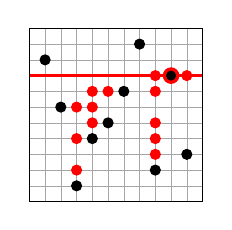
\begin{tikzpicture}[scale=0.2] %8
            \draw[very thin, gray!70] (0,0) grid (11,11);
            
            \draw[teste, line width=1.2pt] (0,8) -- (11,8);
    
            \filldraw[black] (3,1) circle (9pt);
            \filldraw[black] (8,2) circle (9pt);
            \filldraw[black] (10,3) circle (9pt);
            \filldraw[black] (4,4) circle (9pt);
            \filldraw[black] (5,5) circle (9pt);
            \filldraw[black] (2,6) circle (9pt);
            \filldraw[black] (6,7) circle (9pt);
            \filldraw[teste] (9,8) circle (14pt);
            \filldraw[black] (9,8) circle (8pt);
            \filldraw[black] (1,9) circle (9pt);
            \filldraw[black] (7,10) circle (9pt);
            \filldraw[teste] (3,2) circle (9pt);
            \filldraw[teste] (8,3) circle (9pt);
            \filldraw[teste] (3,4) circle (9pt);
            \filldraw[teste] (8,4) circle (9pt);
            \filldraw[teste] (4,5) circle (9pt);
            \filldraw[teste] (8,5) circle (9pt);
            \filldraw[teste] (3,6) circle (9pt);
            \filldraw[teste] (4,6) circle (9pt);
            \filldraw[teste] (4,7) circle (9pt);
            \filldraw[teste] (5,7) circle (9pt);
            \filldraw[teste] (8,7) circle (9pt);
            \filldraw[teste] (8,8) circle (9pt);
            \filldraw[teste] (10,8) circle (9pt);
            \draw[black, line width=0.5pt] (0,0) rectangle (11,11); 
        \end{tikzpicture}
        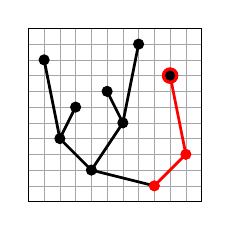
\begin{tikzpicture}[scale=0.2]
            \draw[very thin, gray!70] (0,0) grid (11,11);

            \draw[black, line width=1pt] (8,1) -- (4,2) -- (2,4) -- (3,6);
            \draw[black, line width=1pt] (2,4) -- (1,9);
            \draw[black, line width=1pt] (4,2) -- (6,5) -- (7,10);
            \draw[black, line width=1pt] (6,5) -- (5,7);
            \draw[teste, line width=1pt] (8,1) -- (10,3) -- (9,8);

            \filldraw[teste] (8,1) circle (9pt);
            \filldraw[black] (4,2) circle (9pt);
            \filldraw[teste] (10,3) circle (9pt);
            \filldraw[black] (2,4) circle (9pt);
            \filldraw[black] (6,5) circle (9pt);
            \filldraw[black] (3,6) circle (9pt);
            \filldraw[black] (5,7) circle (9pt);
            \filldraw[teste] (9,8) circle (14pt);
            \filldraw[black] (9,8) circle (8pt);
            \filldraw[black] (1,9) circle (9pt);
            \filldraw[black] (7,10) circle (9pt);
            \draw[black, line width=0.5pt] (0,0) rectangle (11,11);
        \end{tikzpicture}  
        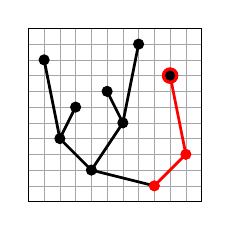
\begin{tikzpicture}[scale=0.2]
            \draw[very thin, gray!70] (0,0) grid (11,11);

            \draw[black, line width=1pt] (8,1) -- (4,2) -- (2,4) -- (3,6);
            \draw[black, line width=1pt] (2,4) -- (1,9);
            \draw[black, line width=1pt] (4,2) -- (6,5) -- (7,10);
            \draw[black, line width=1pt] (6,5) -- (5,7);
            \draw[teste, line width=1pt] (8,1) -- (10,3) -- (9,8);

            \filldraw[teste] (8,1) circle (9pt);
            \filldraw[black] (4,2) circle (9pt);
            \filldraw[teste] (10,3) circle (9pt);
            \filldraw[black] (2,4) circle (9pt);
            \filldraw[black] (6,5) circle (9pt);
            \filldraw[black] (3,6) circle (9pt);
            \filldraw[black] (5,7) circle (9pt);
            \filldraw[teste] (9,8) circle (14pt);
            \filldraw[black] (9,8) circle (8pt);
            \filldraw[black] (1,9) circle (9pt);
            \filldraw[black] (7,10) circle (9pt);
            \draw[black, line width=0.5pt] (0,0) rectangle (11,11);
        \end{tikzpicture}
        \\
        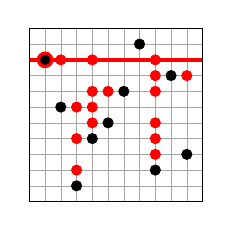
\begin{tikzpicture}[scale=0.2] %9
            \draw[very thin, gray!70] (0,0) grid (11,11);
            
            \draw[teste, line width=1.2pt] (0,9) -- (11,9);
    
            \filldraw[black] (3,1) circle (9pt);
            \filldraw[black] (8,2) circle (9pt);
            \filldraw[black] (10,3) circle (9pt);
            \filldraw[black] (4,4) circle (9pt);
            \filldraw[black] (5,5) circle (9pt);
            \filldraw[black] (2,6) circle (9pt);
            \filldraw[black] (6,7) circle (9pt);
            \filldraw[black] (9,8) circle (9pt);
            \filldraw[teste] (1,9) circle (14pt);
            \filldraw[black] (1,9) circle (8pt);
            \filldraw[black] (7,10) circle (9pt);
            \filldraw[teste] (3,2) circle (9pt);
            \filldraw[teste] (8,3) circle (9pt);
            \filldraw[teste] (3,4) circle (9pt);
            \filldraw[teste] (8,4) circle (9pt);
            \filldraw[teste] (4,5) circle (9pt);
            \filldraw[teste] (8,5) circle (9pt);
            \filldraw[teste] (3,6) circle (9pt);
            \filldraw[teste] (4,6) circle (9pt);
            \filldraw[teste] (4,7) circle (9pt);
            \filldraw[teste] (5,7) circle (9pt);
            \filldraw[teste] (8,7) circle (9pt);
            \filldraw[teste] (8,8) circle (9pt);
            \filldraw[teste] (10,8) circle (9pt);
            \filldraw[teste] (2,9) circle (9pt);
            \filldraw[teste] (4,9) circle (9pt);
            \filldraw[teste] (8,9) circle (9pt);
            \draw[black, line width=0.5pt] (0,0) rectangle (11,11); 
        \end{tikzpicture}
        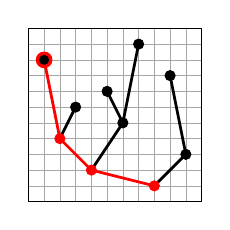
\begin{tikzpicture}[scale=0.2]
            \draw[very thin, gray!70] (0,0) grid (11,11);

            \draw[black, line width=1pt] (2,4) -- (3,6);
            \draw[teste, line width=1pt] (8,1) -- (4,2) -- (2,4) -- (1,9);
            \draw[black, line width=1pt] (4,2) -- (6,5) -- (7,10);
            \draw[black, line width=1pt] (6,5) -- (5,7);
            \draw[black, line width=1pt] (8,1) -- (10,3) -- (9,8);

            \filldraw[teste] (8,1) circle (9pt);
            \filldraw[teste] (4,2) circle (9pt);
            \filldraw[black] (10,3) circle (9pt);
            \filldraw[teste] (2,4) circle (9pt);
            \filldraw[black] (6,5) circle (9pt);
            \filldraw[black] (3,6) circle (9pt);
            \filldraw[black] (5,7) circle (9pt);
            \filldraw[black] (9,8) circle (9pt);
            \filldraw[teste] (1,9) circle (14pt);
            \filldraw[black] (1,9) circle (8pt);
            \filldraw[black] (7,10) circle (9pt);
            \draw[black, line width=0.5pt] (0,0) rectangle (11,11);
        \end{tikzpicture}
        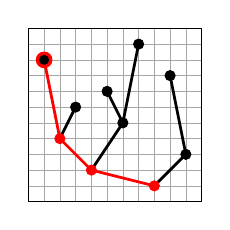
\begin{tikzpicture}[scale=0.2]
            \draw[very thin, gray!70] (0,0) grid (11,11);

            \draw[black, line width=1pt] (2,4) -- (3,6);
            \draw[teste, line width=1pt] (8,1) -- (4,2) -- (2,4) -- (1,9);
            \draw[black, line width=1pt] (4,2) -- (6,5) -- (7,10);
            \draw[black, line width=1pt] (6,5) -- (5,7);
            \draw[black, line width=1pt] (8,1) -- (10,3) -- (9,8);

            \filldraw[teste] (8,1) circle (9pt);
            \filldraw[teste] (4,2) circle (9pt);
            \filldraw[black] (10,3) circle (9pt);
            \filldraw[teste] (2,4) circle (9pt);
            \filldraw[black] (6,5) circle (9pt);
            \filldraw[black] (3,6) circle (9pt);
            \filldraw[black] (5,7) circle (9pt);
            \filldraw[black] (9,8) circle (9pt);
            \filldraw[teste] (1,9) circle (14pt);
            \filldraw[black] (1,9) circle (8pt);
            \filldraw[black] (7,10) circle (9pt);
            \draw[black, line width=0.5pt] (0,0) rectangle (11,11);
        \end{tikzpicture}
        \\
        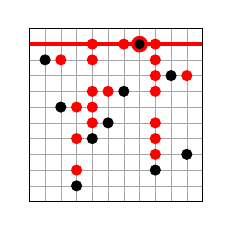
\begin{tikzpicture}[scale=0.2] %10
            \draw[very thin, gray!70] (0,0) grid (11,11);
            
            \draw[teste, line width=1.2pt] (0,10) -- (11,10);
    
            \filldraw[black] (3,1) circle (9pt);
            \filldraw[black] (8,2) circle (9pt);
            \filldraw[black] (10,3) circle (9pt);
            \filldraw[black] (4,4) circle (9pt);
            \filldraw[black] (5,5) circle (9pt);
            \filldraw[black] (2,6) circle (9pt);
            \filldraw[black] (6,7) circle (9pt);
            \filldraw[black] (9,8) circle (9pt);
            \filldraw[black] (1,9) circle (9pt);
            \filldraw[teste] (7,10) circle (14pt);
            \filldraw[black] (7,10) circle (8pt);
            \filldraw[teste] (3,2) circle (9pt);
            \filldraw[teste] (8,3) circle (9pt);
            \filldraw[teste] (3,4) circle (9pt);
            \filldraw[teste] (8,4) circle (9pt);
            \filldraw[teste] (4,5) circle (9pt);
            \filldraw[teste] (8,5) circle (9pt);
            \filldraw[teste] (3,6) circle (9pt);
            \filldraw[teste] (4,6) circle (9pt);
            \filldraw[teste] (4,7) circle (9pt);
            \filldraw[teste] (5,7) circle (9pt);
            \filldraw[teste] (8,7) circle (9pt);
            \filldraw[teste] (8,8) circle (9pt);
            \filldraw[teste] (10,8) circle (9pt);
            \filldraw[teste] (2,9) circle (9pt);
            \filldraw[teste] (4,9) circle (9pt);
            \filldraw[teste] (8,9) circle (9pt);
            \filldraw[teste] (4,10) circle (9pt);
            \filldraw[teste] (8,10) circle (9pt);
            \filldraw[teste] (6,10) circle (9pt);
            \draw[black, line width=0.5pt] (0,0) rectangle (11,11); 
        \end{tikzpicture}
        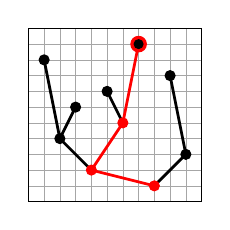
\begin{tikzpicture}[scale=0.2]
            \draw[very thin, gray!70] (0,0) grid (11,11);

            \draw[black, line width=1pt] (2,4) -- (3,6);
            \draw[teste, line width=1pt] (8,1) -- (4,2) -- (6,5) -- (7,10);
            \draw[black, line width=1pt] (4,2) -- (2,4) -- (1,9);
            \draw[black, line width=1pt] (6,5) -- (5,7);
            \draw[black, line width=1pt] (8,1) -- (10,3) -- (9,8);

            \filldraw[teste] (8,1) circle (9pt);
            \filldraw[teste] (4,2) circle (9pt);
            \filldraw[black] (10,3) circle (9pt);
            \filldraw[black] (2,4) circle (9pt);
            \filldraw[teste] (6,5) circle (9pt);
            \filldraw[black] (3,6) circle (9pt);
            \filldraw[black] (5,7) circle (9pt);
            \filldraw[black] (9,8) circle (9pt);
            \filldraw[black] (1,9) circle (9pt);
            \filldraw[teste] (7,10) circle (14pt);
            \filldraw[black] (7,10) circle (8pt);
            \draw[black, line width=0.5pt] (0,0) rectangle (11,11);
        \end{tikzpicture}
        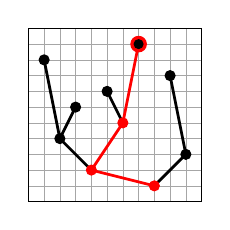
\begin{tikzpicture}[scale=0.2]
            \draw[very thin, gray!70] (0,0) grid (11,11);

            \draw[black, line width=1pt] (2,4) -- (3,6);
            \draw[teste, line width=1pt] (8,1) -- (4,2) -- (6,5) -- (7,10);
            \draw[black, line width=1pt] (4,2) -- (2,4) -- (1,9);
            \draw[black, line width=1pt] (6,5) -- (5,7);
            \draw[black, line width=1pt] (8,1) -- (10,3) -- (9,8);

            \filldraw[teste] (8,1) circle (9pt);
            \filldraw[teste] (4,2) circle (9pt);
            \filldraw[black] (10,3) circle (9pt);
            \filldraw[black] (2,4) circle (9pt);
            \filldraw[teste] (6,5) circle (9pt);
            \filldraw[black] (3,6) circle (9pt);
            \filldraw[black] (5,7) circle (9pt);
            \filldraw[black] (9,8) circle (9pt);
            \filldraw[black] (1,9) circle (9pt);
            \filldraw[teste] (7,10) circle (14pt);
            \filldraw[black] (7,10) circle (8pt);
            \draw[black, line width=0.5pt] (0,0) rectangle (11,11);
        \end{tikzpicture}
    \end{minipage}
    \caption{Na primeira coluna, a execução do guloso futurista para $X = (3,8,10,4,5,2,6,9,1,7)$. Na segunda coluna, a execução de cada acesso na ABB correspondente. Na terceira coluna a ABB final após as rotações executadas depois do acesso da coluna anterior. Note que os nós na linha $r$ do algoritmo guloso da coluna da esquerda são exatamente os nós visitados na coluna do meio, e passíveis de reestruturação na última coluna.}
\label{fig:greedy_em_ABB}
\end{figure}

Como mostrado no Lema~\ref{lema:ASS_vira_visao_geometrica}, e evidenciado pela Figura~\ref{fig:greedy_em_ABB}, é possível a partir unicamente do conjunto de pontos $P$ resultante da execução do algoritmo guloso futurista para uma sequência $X$ de acessos construir os passos que devem ser executados para um algoritmo de busca executar todos os acessos de $X$ apenas visitando os nós representados pelos pontos de $P$. 

Note que para isso foi necessário inicializar a árvore com os nós ordenados pelo primeiro acesso de cada nó e também foi necessário saber a próxima visita aos nós para ter a informação de como reestruturar a ABB durante os acessos de maneira a apenas visitar os nós propostos. Assim, apesar do guloso futurista ser um algoritmo online, a princípio a sua tradução para um algoritmo de busca em ABB necessita de mais informação e, portanto, é offline.

Demaine et al. \cite{geometry_of_bst} provaram que utilizando uma estrutura abstrata de dados chamada árvore split que implementa as operações maketree e split no modelo de computação adotado é possível converter um algoritmo online do contexto de conjunto de pontos arboreamente satisfeitos em um algoritmo online do contexto de buscas em ABBs com custo extra limitado por um fator constante. A ideia central é evitar tomar decisões sobre como dispor os nós na ABB e armazenar esses nós em uma árvore split. Dessa maneira é possível utilizar a operação split no futuro quando for necessário visitar um dos nós presentes nesta árvore split. Essa prova é bastante enigmática e de difícil compreensão, envolvendo uma série de estruturas de dados como árvores treap, árvores rubro-negras e árvores 2-3-4. Para esse texto, basta perceber que é possível converter o algoritmo guloso futurista em um algoritmo online de busca em ABBs sem aumento significativo do seu custo.

Embora o algoritmo garanta encontrar um superconjunto $P$ arboreamente satisfeito de $P_X$, o guloso futurista não garante que $|P| = \minASS(P_X)$. Veja a Figura~\ref{fig:greedy_subotimo}.

\begin{comment}
\begin{figure}
    \centering
    
    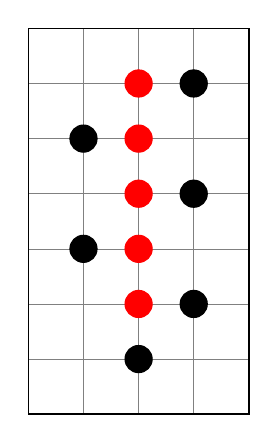
\begin{tikzpicture}[scale=0.7]
        \draw[very thin, gray] (0,0) grid (4,7);

        \filldraw[black] (2,1) circle (7pt);
        \filldraw[black] (3,2) circle (7pt);
        \filldraw[black] (1,3) circle (7pt);
        \filldraw[black] (3,4) circle (7pt);
        \filldraw[black] (1,5) circle (7pt);
        \filldraw[black] (3,6) circle (7pt);
        \filldraw[teste] (2,2) circle (7pt);
        \filldraw[teste] (2,3) circle (7pt);
        \filldraw[teste] (2,4) circle (7pt);
        \filldraw[teste] (2,5) circle (7pt);
        \filldraw[teste] (2,6) circle (7pt);
        
        \draw[black, line width=0.5pt] (0,0) rectangle (4,7);
    \end{tikzpicture}
    \\
    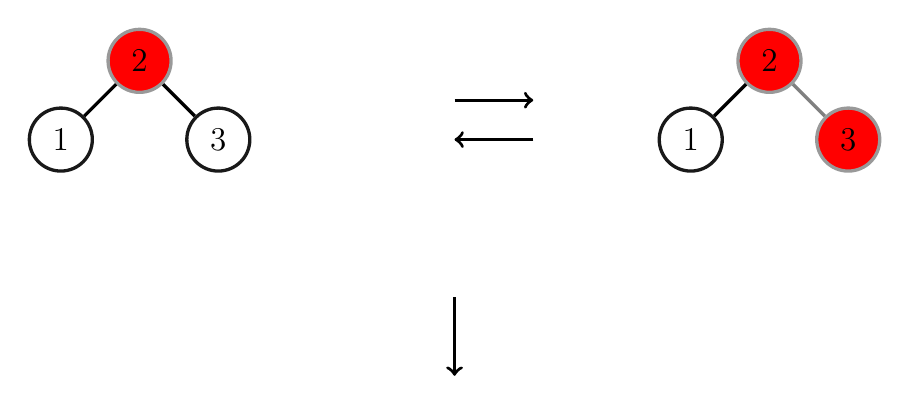
\begin{tikzpicture}[
        level distance=1cm,
        level 1/.style={sibling distance=2cm},
        every node/.style={circle, draw=black!90, very thick, minimum size=8mm, inner sep=0pt, font=\large},
        edge from parent/.style={draw, solid, very thick},
        edge from parent path={(\tikzparentnode) -- (\tikzchildnode)},
        nodeteste/.style={circle, draw=gray!80, solid, minimum size=8mm, inner sep=0pt, font=\large, fill=teste},
        edgeGray/.style={circle, draw=gray}
        ]
        \node [nodeteste] {2}
          child {node {1}}
          child {node {3}};
    
        \draw[->, very thick] (4,-0.5) -- (5,-0.5);
        \draw[->, very thick] (5,-1) -- (4,-1);
        \draw[->, very thick] (4,-3) -- (4,-4);
    
        \begin{scope}[xshift=8cm] % Desloca a segunda árvore para a direita
        \node [nodeteste] {2}
            child {node {1}}
            child [edgeGray] {node [nodeteste] {3}};
        \end{scope}
    \end{tikzpicture}
    \\
    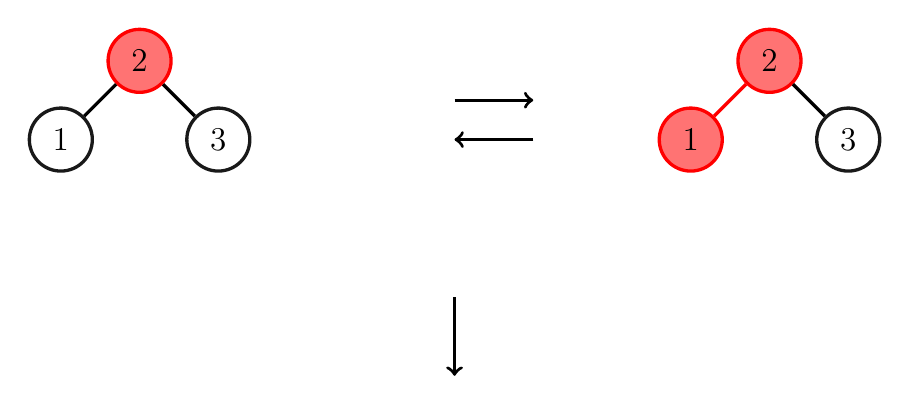
\begin{tikzpicture}[
        level distance=1cm,
        level 1/.style={sibling distance=2cm},
        every node/.style={circle, draw=black!90, very thick, minimum size=8mm, inner sep=0pt, font=\large},
        edge from parent/.style={draw, solid, very thick},
        edge from parent path={(\tikzparentnode) -- (\tikzchildnode)},
        nodeteste/.style={circle, draw=teste, solid, minimum size=8mm, inner sep=0pt, font=\large, fill=teste!55}
        ]
        \node [nodeteste] {2}
          child {node {1}}
          child {node {3}};
    
        \draw[->, very thick] (4,-0.5) -- (5,-0.5);
        \draw[->, very thick] (5,-1) -- (4,-1);
        \draw[->, very thick] (4,-3) -- (4,-4);
    
        \begin{scope}[xshift=8cm] % Desloca a segunda árvore para a direita
        \node [nodeteste] {2}
            child [nodeteste] {node [nodeteste] {1}}
            child {node {3}};
        \end{scope}
    \end{tikzpicture}
    \\
    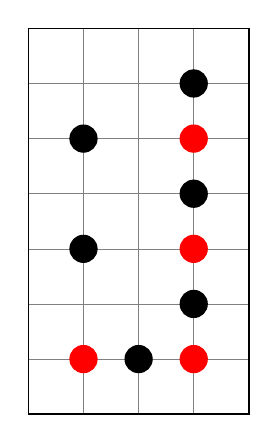
\begin{tikzpicture}[scale=0.7]
        \draw[very thin, gray] (0,0) grid (4,7);
        
        \filldraw[black] (2,1) circle (7pt);
        \filldraw[black] (3,2) circle (7pt);
        \filldraw[black] (1,3) circle (7pt);
        \filldraw[black] (3,4) circle (7pt);
        \filldraw[black] (1,5) circle (7pt);
        \filldraw[black] (3,6) circle (7pt);
        \filldraw[teste] (1,1) circle (7pt);
        \filldraw[teste] (3,1) circle (7pt);
        \filldraw[teste] (3,3) circle (7pt);
        \filldraw[teste] (3,5) circle (7pt);
        
        \draw[black, line width=0.5pt] (0,0) rectangle (4,7);
    \end{tikzpicture}
    \\
    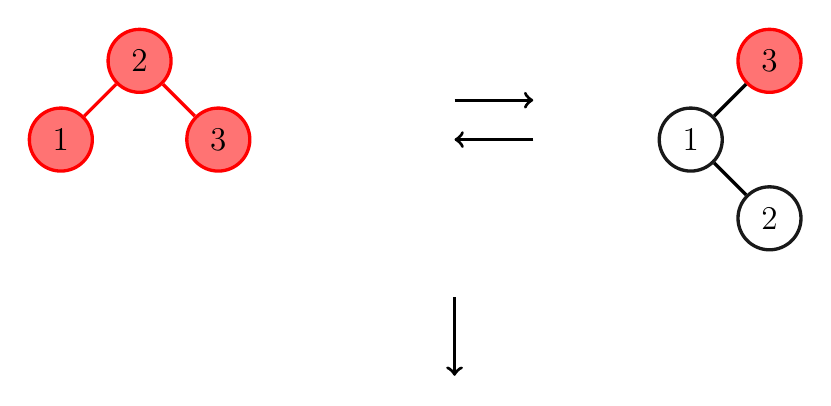
\begin{tikzpicture}[
        level distance=1cm,
        level 1/.style={sibling distance=2cm},
        every node/.style={circle, draw=black!90, very thick, minimum size=8mm, inner sep=0pt, font=\large},
        edge from parent/.style={draw, solid, very thick},
        edge from parent path={(\tikzparentnode) -- (\tikzchildnode)},
        nodeteste/.style={circle, draw=teste, solid, minimum size=8mm, inner sep=0pt, font=\large, fill=teste!55}
        ]
        \node [nodeteste] {2}
          child [nodeteste] {node [nodeteste] {1}}
          child [nodeteste] {node [nodeteste] {3}};
    
        \draw[->, very thick] (4,-0.5) -- (5,-0.5);
        \draw[->, very thick] (5,-1) -- (4,-1);
        \draw[->, very thick] (4,-3) -- (4,-4);
    
        \begin{scope}[xshift=8cm] % Desloca a segunda árvore para a direita
        \node [nodeteste] {3}
            child {node {1}
                child[missing] {}
                child {node {2}}}
            child[missing] {};
        \end{scope}
    \end{tikzpicture}
    \\
    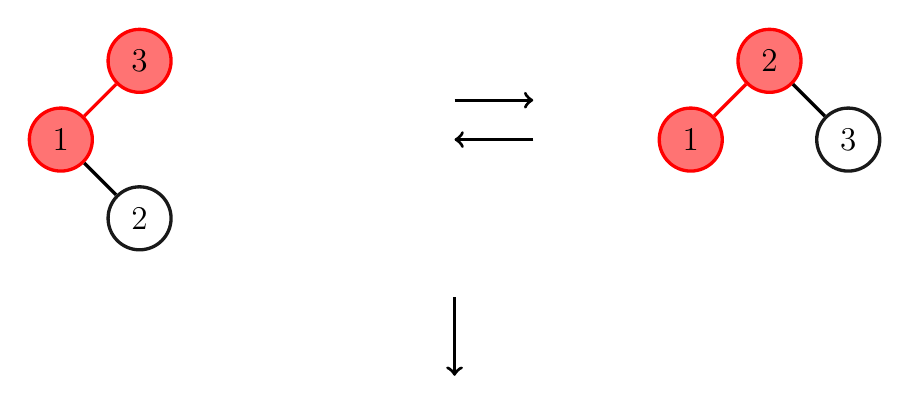
\begin{tikzpicture}[
        level distance=1cm,
        level 1/.style={sibling distance=2cm},
        every node/.style={circle, draw=black!90, very thick, minimum size=8mm, inner sep=0pt, font=\large},
        edge from parent/.style={draw, solid, very thick},
        edge from parent path={(\tikzparentnode) -- (\tikzchildnode)},
        nodeteste/.style={circle, draw=teste, solid, minimum size=8mm, inner sep=0pt, font=\large, fill=teste!55},
        nodeBlack/.style={circle, draw=black, solid, minimum size=8mm, inner sep=0pt}
        ]
        \node [nodeteste] {3}
            child [nodeteste] {node [nodeteste] {1}
                child[missing] {}
                child [nodeBlack] {node {2}}}
            child[missing] {};
    
        \draw[->, very thick] (4,-0.5) -- (5,-0.5);
        \draw[->, very thick] (5,-1) -- (4,-1);
        \draw[->, very thick] (4,-3) -- (4,-4);
    
        \begin{scope}[xshift=8cm] % Desloca a segunda árvore para a direita
        \node [nodeteste] {2}
            child [nodeteste] {node [nodeteste] {1}}
            child {node {3}};
        \end{scope}
    \end{tikzpicture}
    \caption{Em preto, os pontos de $P_X$ para uma sequência $X = (2,3,1,3,1,3)$ de acessos. À esquerda, o conjunto de pontos produzidos pelo Guloso futurista. À direita, o menor conjunto arboreamente satisfeito para $P_X$, de tamanho \minASS$(P_X)$.}
\label{fig:greedy_subotimo}
\end{figure}
\end{comment}

\begin{figure}
    \centering
    \includegraphics[scale=0.8]{imagens/guloso_subotimo.pdf}
    \caption{Em cima, o conjunto de pontos $P$ produzido pelo algoritmo guloso futurista para a sequência $X = (2,3,1,3,1,3)$ de acessos. À direita desse conjunto de pontos está a ABB correspondente onde as buscas são feitas com os nós visitados em cada busca destacados. Abaixo, um conjunto de pontos $P'$ com tamanho \minASS$(P_X)$. À direita desse conjunto está a ABB correspondente onde os nós visitados em cada acesso estão destacados.}
\label{fig:greedy_subotimo}
\end{figure}

Analisando o caso acima, perceba que o guloso futurista, por ser um algoritmo online, sempre assume que a primeira chave buscada é a chave da raiz da árvore inicial em sua execução refletida no contexto de ABBs. Após o acesso à chave 2, todas as buscas se alternam entre as chaves 1 e 3, porém a chave 2 não é mais buscada. Assim, fica óbvio perceber que o nó com chave 2 deveria ser retirado do caminho das duas folhas, porém pelo algoritmo fazer decisões gulosas locais, para ele rotacionar o nó com chave 2 para baixo é necessário que ele visite todos os nós da árvore e isso não pode ocorrer. No caso ótimo é exatamente isso que acontece: o algoritmo visita todos os nós no início e já rotaciona o nó com chave 2 para a folha, garantindo assim que esse nó não vai ser visitado de maneira desnecessária no futuro.

Para uma sequência $X$ de acessos com tamanho $m$, formada por uma busca à chave 2 e depois buscas alternadas entre as chaves 1 e 3, é possível notar que o custo do algoritmo guloso futurista é $\OPT(X)$ + $m$/2.

O pior caso encontrado do algoritmo guloso futurista foi proposto por Munro~\cite{munro}. Esse caso acontece quando o algoritmo guloso futurista busca, em uma ABB completa, as chaves na ordem da sequência bit-reversa e em seguida busca apenas as chaves seguindo a mesma sequência. Munro conjecturou que o custo do guloso futurista é $\OPT(X)$ + $\Oh(m)$ para toda sequência $X$ de acessos. Essa sequência particular apresentada por Munro é de extrema importância para o estudo de delimitações de custo em algoritmos de busca em ABBs que permitem rotações e será explicada mais à frente no Capítulo~\ref{cap:wilber}.

Se provada a conjectura de Munro, que o custo do guloso futurista é $\OPT(X)$ + $\Oh(m)$ para toda sequência $X$ de acessos, como $\OPT(X) \geq m$, então prova-se também que o algoritmo guloso futurista tem custo $\Oh(\OPT(X))$. Assim, o algoritmo de busca em ABBs resultante da conversão do algoritmo guloso futurista para o contexto de ABBs possuiria também custo $\Oh(\OPT(X))$ e seria dinamicamente ótimo. Ou seja, essa conjectura de Munro implica que a implementação online de Demaine et al.~\cite{geometry_of_bst} do guloso futurista é dinamicamente ótima.